OpenID standardin ensimmäisen version on kehittänyt toukokuussa 2005 Brad Fitzpatrick \cite{openid}. Tuoreimman 2.0 version kehitys aloitettiin 2007 ja sen kehitys on edelleen aktiivista. OpenID on SAMLia rajoitetumpi protokolla, koska se tarjoaa vain käyttäjän tunnistautumisen. Sen tavoite on saman käyttäjätunnuksen käytön mahdollistaminen eri web-palveluissa. Nykyään sen kehityksestä vastaa \mbox{OpenID} Foundation -säätiö, jonka jäseniä ovat mm. Faceobok, Google ja Microsoft \cite{openid_foundation}.

OpenID-palveluntarjoaja tarjoaa päätepisteen (endpoint), jota web-palvelut käyttävät tunnistautumiseen. Tunnistautumiseen voidaan käyttää kahta erilaista virtausta (flow). Suunnatussa identiteetin (directed identity) virtauksessa käyttäjä valitsee palveluntarjoajan, jonka kautta kirjautuminen suoritetaan \cite{openid}. Väitetyn identiteetin (claimed identity) virtauksessa web-palvelu hakee päätepisteen annetun OpenID\--tun\-nis\-teen perusteella \cite{openid}. Virtaukset eroavat toisistaan vain vaiheessa, jossa etsitään päätepiste. Kuvassa \ref{openid_flow} on esitetty OpenID-kirjautumisen vaiheet.

\begin{figure}[ht]
\centering
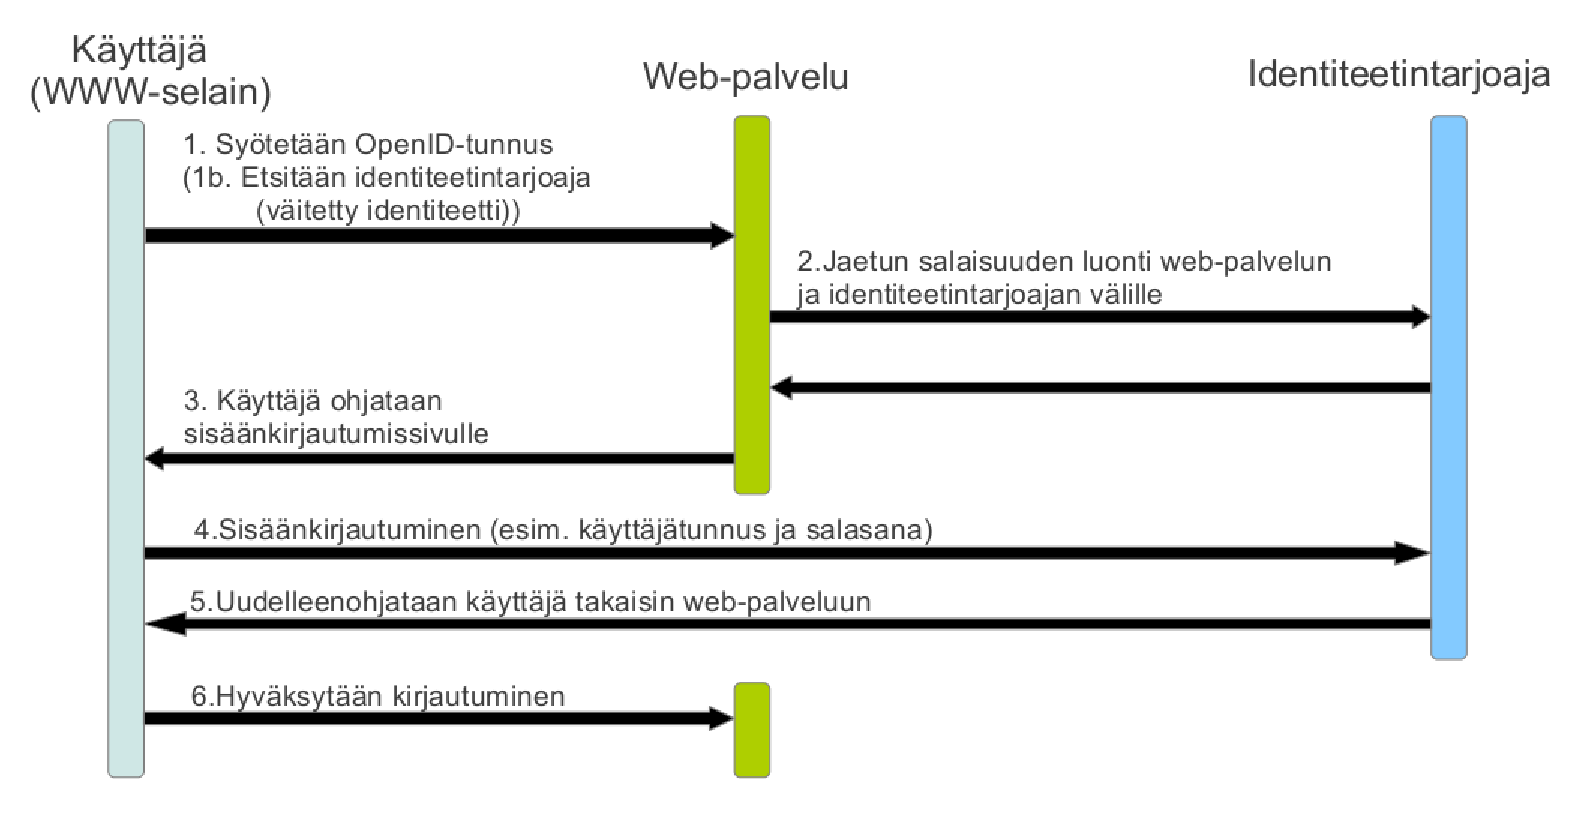
\includegraphics[width=\textwidth]{teknologiat/protokollat/openid.eps}
\caption{OpenID kirjautumisen vaiheet \cite{openid}.}%
\label{openid_flow}
\end{figure}

OpenID:n suhteen odotukset olivat alkujaan suuria, mutta myöhemmin into protokollan ympärillä on laantunut. Esimerkiksi Microsoftin vuonna 2008 aloittama OpenID-kokeilu lopetettiin elokuussa 2009 ja Microsoft on siirtynyt käyttämään omaa tunnistautumistoteutusta \cite{openid_microsoft}. Myös protokollaan liittyvät turvallisuushuolet ovat kasvaneet viime aikoina, koska se koetaan alttiiksi erilaisille kalastelu yms hyökkäyksille \cite{billion_keys}.

Yleiset OpenID-kir\-jau\-tu\-mis\-si\-vut on korvattu eri palveluntarjoajien kirjautumissivuilla, koska käyttäjätutkimusten mukaan käyttäjät eivät tunne OpenID:tä, mutta tuntevat palveluntarjoajan kuten Googlen tai Yahoon \cite{refuse_sso}. Näin ollen käyttäjät eivät tiedä kirjautuvansa OpenID:llä palveluun, johon kirjaudutaan Googlen tunnuksilla. Myös alkuperäinen ajatus siitä, että kuka tahansa voi toimia identiteetintarjoajana, on osoittatunut toimimattomaksi, koska web-palveluiden ylläpitäjät haluavat luottaa päätepisteisiin, joiden kautta heidän palveluun voi kirjautua \cite{refuse_sso}.

OpenID:tä lähellä on erillinen OAuth-protokolla, jonka toteutus aloitettiin, kun huomattiin, että OpenID ei sovellu kaikkiin tapauksiin. OpenID varmistaa vain sen, että käyttäjä on se joka väittää olevansa, mutta se ei ota kantaa käyttäjän pääsyoikeuksiin. OpenID säätiö on julkaisemassa myös uutta OpenID Connect -määritelmää, joka lisää protokollaan myös pääsynvalvonnan \cite{distributed_web_security}. Sen kehitys on kuitenkin vielä niin varhaisessa määrittelyvaiheessa, että sen käyttö tämän tutkielman puitteissa ei ole mielekästä. Sen sijaan OAuth-protokolla, johon myös tuleva OpenID Connect -protokolla perustuu, esitellään seuraavassa aliluvussa.